\section{The Proposed Model}

In this section, we present the proposed  model that leverages  Meta-path based Context for RECommendation, called \textbf{MCRec}.
%Our MCRec model characterizes the interaction between users and items with the incorporation of meta-paths as context.


%extends the neural collaborative filtering framework~\cite{he2017neural} by incorporating meta-path based context. The meta-path based context is first modeled by a hierarchical embedding method, and then improved with the co-attention mechanism.


\subsection{Model Overview}
Different from existing HIN based recommendation models, which only learn the representations for users and items,  we explicitly incorporate meta-paths as the context  in an interaction between a user and an item.
Instead of modeling the two-way interaction $\langle user, item \rangle$, we aim to characterize a three-way interaction
$\langle \emph{user}$, \emph{\text{meta-paths}}, $\emph{item} \rangle$.
For learning a better interaction function that generates the recommendations, we learn the representations (\ie embedding) for users, items and their interaction contexts, which is the aggregated meta-paths.
We present the overall architecture for the proposed model in Fig.~\ref{fig-framework-model}.
As we can see, besides the components for learning user and item embeddings, the most important part lies in the embedding of \emph{meta-path based context}. The meta-path based context is first modeled into a low-dimensional embedding using a hierarchical neural network.
With the initially learned embeddings for users, items and meta-path based context, the co-attention mechanism further improves the three representations through alternative enhancement. Due to the incorporation of  meta-path based context, our model is expected to yield a better performance and also improve the interpretability for recommendation results.

\begin{figure}
  \centering
  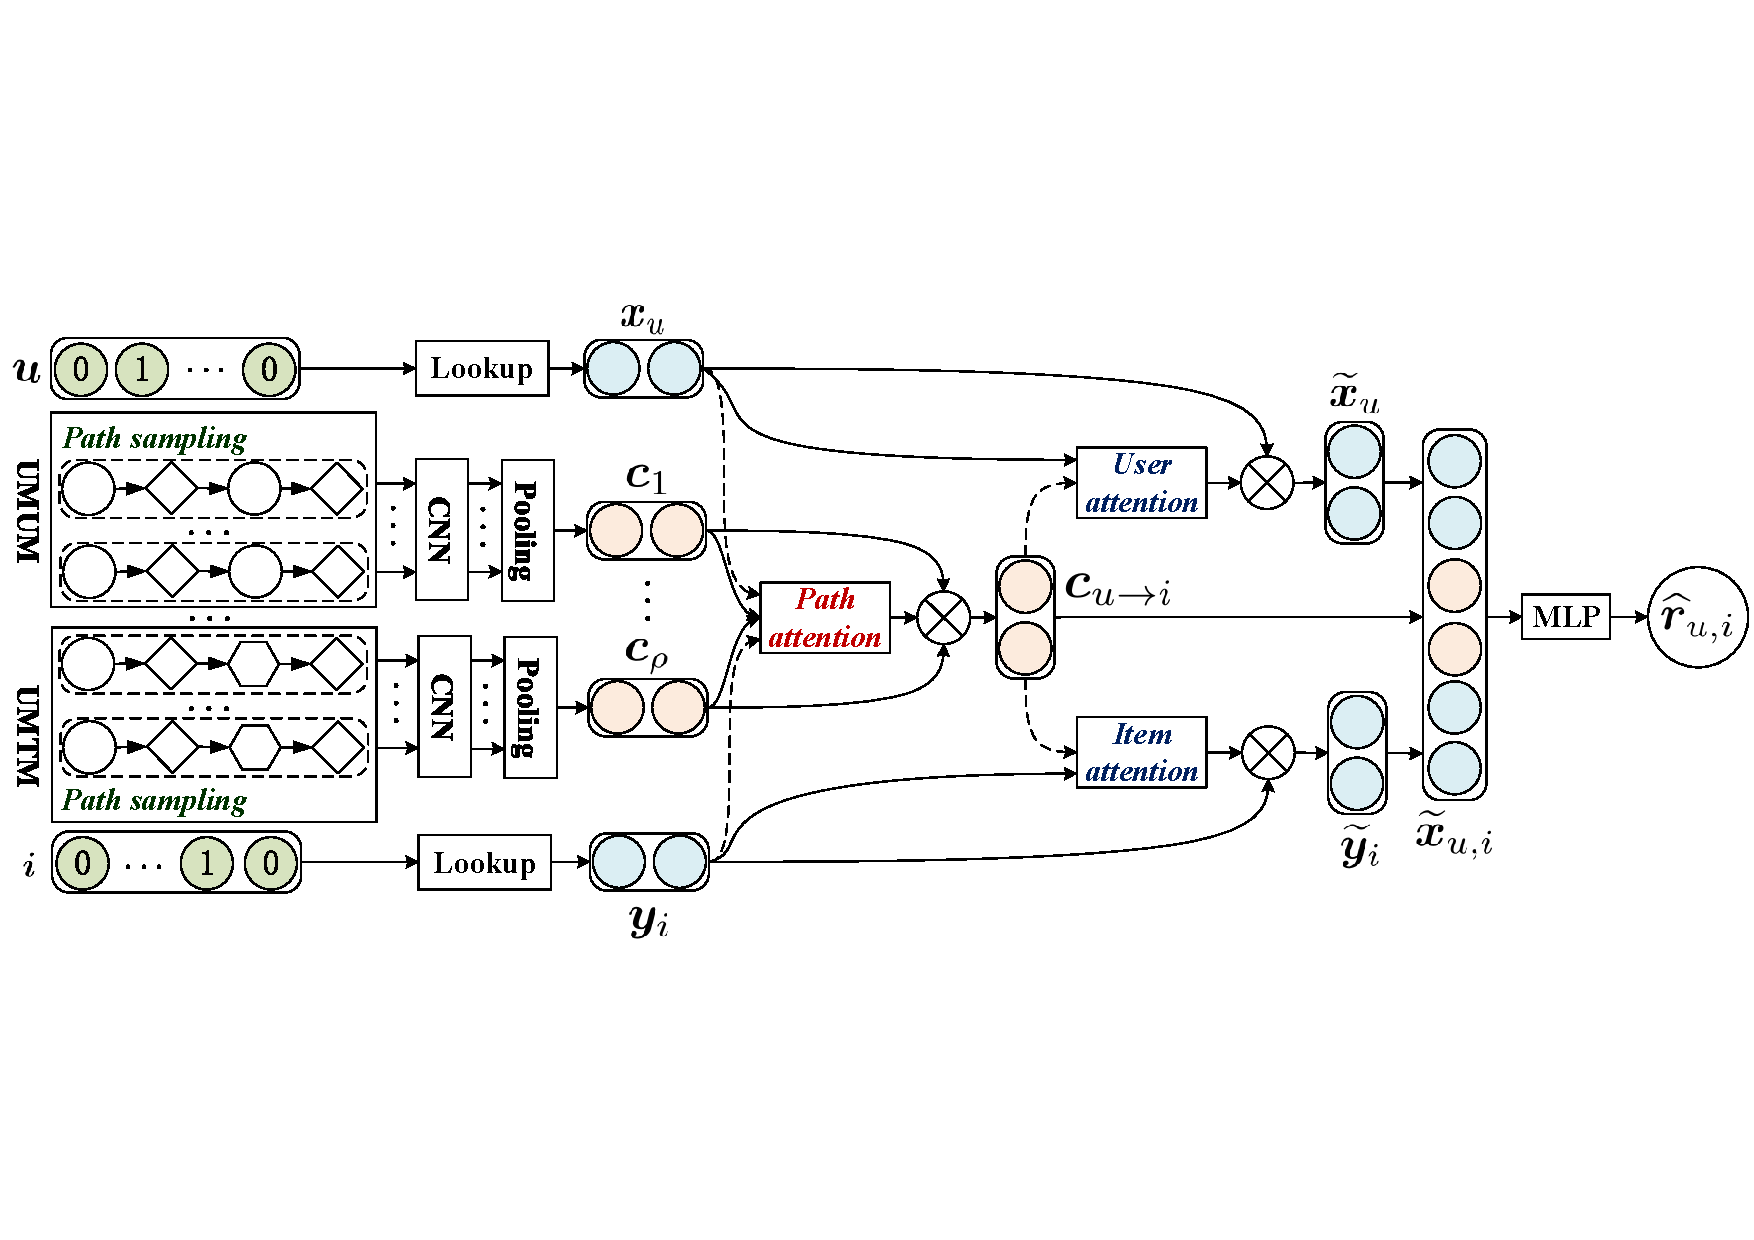
\includegraphics[width=8.5cm]{image/framework_model.pdf}\\
  \caption{The overall architecture of the proposed model.}\label{fig-framework-model}
\end{figure}

%we  propose a \emph{M}eta-path based \emph{C}context embedding model for top-N \emph{Rec}ommendation (called MCRec). The basic idea of MCRec is that, except the embedding of users and items, MCRec learns the context embedding of a $\langle user, item \rangle$ pair through fusing the meta-path embeddings connecting the user and item, and then exploits the correlations of the embeddings of users, items,  and their context. As illustrated in Fig.~\ref{fig-framework-model}, MCRec includes two main components: learn embeddings of users, items, and their context, and fuse embeddings. In the context embedding phrase, MCRec first learns path embedding for each meta-path connecting a user $u$ and item $i$, and then fuse these multiple path embeddings for the context of the $\langle u, i\rangle$ with the help of the embeddings of user $u$ and item $i$. In the embeddings fusing phrase,  the embeddings of user $u$, item $i$, and  $\langle u, i\rangle$ context enhance each other with a co-attention network. In the following sections, we will present the details of these components.

\subsection{User and Item Embedding}

Following~\cite{he2017neural}, we set up a lookup layer to transform the one-hot representations of users and items into
 low-dimensional dense vectors, called \emph{embeddings}. Formally, given a user-item pair $\langle u, i \rangle$, let
 $\mathbf{p}_u \in \mathbb{R}^{|\mathcal{U}| \times 1}$ and $\mathbf{q}_i \in \mathbb{R}^{|\mathcal{I}| \times 1}$ denote their one-hot representations.  The lookup layers correspond to two parameter matrices $\mathbf{P} \in \mathbb{R}^{|\mathcal{U}| \times d}$ and $\mathbf{Q} \in \mathbb{R}^{|\mathcal{I}| \times d  }$, which store the latent factors for users and items respectively.  Here $d$ is the dimension size of user and item embeddings, and $|\mathcal{U}|$ and $|\mathcal{I}|$ are the total number of users and items respectively.
 The lookup operation is implemented as follows:
 \begin{eqnarray}
\mathbf{x}_u &=& \mathbf{P}^{\top} \cdot \mathbf{p}_u, \label{equ-userembedding}\\
\mathbf{y}_i &=& \mathbf{Q}^{\top} \cdot \mathbf{q}_i. \label{equ-itemembedding}
\end{eqnarray}

%Similar to previous HIN based recommendation models, the MCRec first learns the embedding of users and items, as shown in two sides of Fig. \ref{fig-framework-model}. The proposed model accepts a user-item pair $\langle u, i \rangle$ as input. We represent the involved user $u$ and item $i$ as one-hot vectors corresponding to a unique index key belonging to user $u$ and item $i$, $\eg$ $\mathbf{p}_u \in \mathbb{R}^{|\mathcal{U}| \times 1}$ and $\mathbf{q}_i \in \mathbb{R}^{|\mathcal{I}| \times 1}$. In the embedding layer, these one-hot vectors can be transformed to low-dimensional real-value representations. In order to embed users and items, we introduce two parameter matrices $\mathbf{P} \in \mathbb{R}^{d \times |\mathcal{U}|}$ and $\mathbf{Q} \in \mathbb{R}^{d \times |\mathcal{I}|}$ which store the latent factors for users and items respectively. Here $d$ is the dimension of user and item embeddings, while $|\mathcal{U}|$ and $|\mathcal{I}|$ are the total number of users and items respectively. By applying a lookup layer, we can obtain the embeddings of users and items as follows:


\subsection{Characterizing Meta-path based Context for Interaction}
A major novelty of our work is to explicitly characterize meta-path based context for improving the modeling of the  interaction.
In this part, we first study how to generate high-quality path instances, and then present how to learn effective representations (\ie embeddings) for meta-path based context.

%Different from HIN based recommendation models and HIN embedding methods, we designs a novel meta-path based context embedding to exploit the rich semantic interactions between users and items through fusing multiple path embeddings, as shown in the middle of  Fig. \ref{fig-framework-model}. The MCRec first samples several path instances based on a given meta-path with a novel heuristic random walk strategy, and then embeds these path instances with a CNN layer. After that, the embedding of this meta-path can be obtained through fusing these path instance embeddings. Finally, we give a naive context embedding strategy to fuse multiple meta-path embeddings.

\subsubsection{Sampling Path Instances via Priority based Random Walk based on Meta-paths}
Existing HIN embedding models mainly adopt a meta-path guided random walk strategy to generate path instances~\cite{dong2017metapath2vec}, relying on a uniform sampling over the out-going nodes.
However, the path instances generated by such a simple random walk strategy are usually of low quality and even accompanied with much noise, which makes the sampling strategy unsuitable for recommendation.
Intuitively, at each step, the walker should  wander to a neighbor of a higher ``priority'' score with a larger probability, since such an out-going node can reflect more reliable semantics by forming a more close link. Hence, the key problem is how to define the priority score of an out-going node.
Inspired by the tricks for training neural networks~\cite{he2017neural,hinton2012better}, we propose to use a similar \emph{pretrain} technique to measure the priority degree of each candidate out-going nodes.  The basic idea is to first learn a latent vector for each node with historical user-item interaction records by using traditional matrix factorization method without meta-path information. Then, we can measure the priority degree by the similarity between the current node and candidate out-going nodes.  Such a priority score directly reflects the association degree between two nodes. To pretrain the latent factors for all the entities in HIN, we train the feature based matrix factorization framework SVDFeature~\cite{chen2012svdfeature}, adapted to implicit feedback with the pairwise loss in~\cite{rendle2009bpr}, on all the available historical interaction records.  SVDFeature is able to characterize various kinds of context information. We can incorporate the entities from HIN related to an interaction as the context of a training instance. With the learned latent factors, we can compute the pairwise similarities between two consecutive nodes along a path instance, and then average these similarities for ranking the candidate path instances. Finally, given a meta-path, we only keep top $K$ path instances with the highest average similarities.

%In our recommendation task, users and items are the two core entity types, and the key part is the out-going link of the forms $user \rightarrow item$ and $item \rightarrow user$.
%We adopt the widely used Bayesian Personalized Ranking model (BPR) with implicit feedback to learn both user and  item latent factors.
%Given a user node and item node, we use the inner product between their corresponding latent factors as the link importance.
%For each walk with the forms $user \rightarrow item$ and $item \rightarrow user$, we sample the candidate node according to their link importance
%with the current node.  Note that we don't consider compute the importance for links with  other forms, \eg $item  \rightarrow type $ or $user  \rightarrow type$, since we have found that the links between user and item nodes play the key role in generating high-quality path instances.
%While, our approach can be easily extended to compute a full-path importance score by learning a latent factor for each kind of entities, \eg using Factorization Machine~\cite{rendle2010factorization}.  Given a meta-path, for efficiency consideration, we only keep top $K$ path instances with the highest average link importance.

%In order to learn the embedding of a user-item pair, we need to sample some path instances connect the user and item. In recent HIN embedding models \cite{}, meta-path based random walk strategy is widely employed to extract path instances, since meta-path can effectively extract features and embody rich semantics \cite{}. However?the path instances generated by a simple meta-path based random walk strategy usually be low-quality, accompanied with much noise, which makes this strategy not suitable for recommendation. We know that, in RS, there are a huge number of user-item pairs, so we can only sample a small number of path instances for each user-item pair. For the specific requirement of RS, we propose a novel preference-guided random walk strategy based on meta-path to sample a small number of high-quality path instances that can effectively represent structure information of nodes. The basic idea is that we can let walkers wander to neighbors with the higher preference degree, since each node has  more close relation with its preferring neighbors. The preference degree can be simulated by the product of the latent factors of two nodes, where the latent factors can be calculated by factorizing the relation matrix of the adjacent two node types. Concretely, a walker wanders along the given meta-path, and selects the top-$l$ candidate neighbors with high preference degree in each step. After that, we select the top-$K$ path instances with high average of preference degree as samples. Although it is time-consuming for calculating the preference degree, the process can be done offline. In addition, we do not need to calculate the preference degree in each step. We just need to do preference selection on the ``user-item'' relation, since this relation is more important for recommendation. Experiments also validate that MCRec can achieve good performance with only 5 sampled path instances for each user-item pair.

\subsubsection{Meta-path based Context Embedding} After obtaining path instances from multiple meta-paths, we continue to study how to model these
meta-path based context as an informative embedding. Our method naturally follows a hierarchical structure: embedding a single path instance $\rightarrow$  embedding a single meta-path $\rightarrow$  embedding the aggregate meta-paths.

\paratitle{Path Instance Embedding}.  A path instance is essentially a sequence of entity nodes.
To embed such a node sequence into a low-dimensional vector, many methods can apply. Here, we adopt the commonly used Convolution Neural Network (CNN) to deal with sequences of variable lengths. Formally, given a path $p$ from some meta-path $\rho$, let $\mathbf{X}^{p} \in \mathbb{R}^{L \times d}$ denote the embedding matrix formed by concatenating node embeddings, where  $L$ is the length of the path instance and $d$ is the embedding dimension for entities. The structure of CNN consists of a convolution layer (producing new features with the convolution operation) and a max pooling layer. We learn the embedding of a path instance $p$ using CNN as follows:

\begin{equation} \label{equ-pathembedding}
\mathbf{h}_p = CNN(\mathbf{X}^{p}; \mathbf{\Theta})
\end{equation}
where $\mathbf{X}^{p}$ denotes the matrix of the path instance $p$ and $\mathbf{\Theta}$ denotes all the related parameters in CNNs.
%where $*$ denotes the convolution operator, $b_j$ is a bias term and $f$ is an activation function. In our work, we use Rectified Linear Units (ReLU) \cite{nair2010rectified}, which yields better than tanh unit and sigmoid unit in our empirical results. The ReLU unit is defined as follows.
%\begin{equation}\label{equ-relu}
%f(x) = max\{0, x\}.
%\end{equation}

\paratitle{Meta-path Embedding}. Since a meta-path can produce multiple path instances,  we further apply the max pooling operation to derive the embedding for a meta-path. Let $\{\mathbf{h}_p\}_{p = 1}^{K}$ denote the embeddings for the $K$ selected path instances from meta-path $\rho$.
The embedding $\mathbf{c}_\rho$ for meta-path $\rho$ can be given

\begin{equation} \label{equ-pooling}
\mathbf{c}_\rho = \text{max-pooling}(\{\mathbf{h}_p\}_{p = 1}^{K}).
\end{equation}
Our max pooling operation is carried out over $K$ path instance embeddings, which aim to capture the important dimension features from multiple path instances.

\paratitle{Simple Average Embedding for Meta-path based Context}. Finally, we apply the average pooling operation to derive the embedding for modeling the aggregate meta-path based context

\begin{equation} \label{equ-avg}
\mathbf{c}_{u \rightarrow i} = \frac{1}{|\mathcal{M}_{u \rightarrow i}|}\sum_{\rho \in \mathcal{M}_{u \rightarrow i} }\mathbf{c}_{\rho},
\end{equation}
where $\mathbf{c}_{u \rightarrow i}$ is the embedding for meta-path based context and $\mathcal{M}_{u \rightarrow i}$ is the set of the considered meta-paths for the current interaction. In this naive embedding method, each meta-path indeed receives equal attention, and
the representation of meta-path based context fully depends on the generated path instances.
It does not incorporate the involved user and item into consideration, which lacks the ability of capturing varying semantics from meta-paths in different interaction scenarios.

\subsection{Improving Embeddings for Interaction via Co-Attention Mechanism}
%Above, the embedding learning of meta-path based context does not take the involved user-item pair into consideration, which can't effectively capture the varying semantics of a  meta-path in different interaction scenarios.
%The above embedding method
Intuitively, different users are likely to have different preferences over the meta-paths.
Even for the same user, a meta-path may have varying semantics in her multiple interactions with different items.
A good embedding method for modeling meta-path based context should be interaction-specific,
which is able to provide highly discriminative semantics in various complicated recommendation scenarios.
Furthermore, in a user-item interaction, meta-paths provide important context information, and hence the involved user and item are likely to be affected
by such interaction context, too.
Based on these discussions, if we could improve the embeddings of users, items and meta-paths in a mutual enhancement way,
it may be possible to  develop a more effective representation learning method.
Inspired by the recent progress of attention mechanism made in computer vision and natural language processing~\cite{xu2015show,phan2017neupl},
we propose a novel co-attention mechanism to achieve this goal.


%could fully model the dependence between a user, an item and meta-paths in an interaction,  we may be able to develop an more effective representation learning method. Inspired by the recent progress of attention mechanism made in computer vision and natural language processing~\cite{mnih2014recurrent,phan2017neupl}, we propose a novel co-attention mechanism to achieve our goal.
%we should jointly learn the embeddings for meta-path, users, and items.
%the meta-path based context should be modeled accordingly in different interactions
%In this way, the embedding for modeling meta-path based context


\subsubsection{Attention for Meta-path based Context}
Since different meta-paths may have different semantics in an interaction, we learn the interaction-specific attention weights over meta-paths conditioned on the involved user and item.  Given the user embedding $\mathbf{x}_u$, item embedding $\mathbf{y}_i$, the  context embedding $\mathbf{c}_\rho$ for  a meta-path $\rho$, we adopt a two-layer architecture to implement the attention

\begin{eqnarray}
\bm{\alpha}^{(1)}_{u, i, \rho} &=& f(\mathbf{W}^{(1)}_u\mathbf{x}_u + \mathbf{W}^{(1)}_i\mathbf{y}_i + \mathbf{W}^{(1)}_{\rho}\mathbf{c}_{\rho} + \mathbf{b}^{(1)}), \label{equ-attention1}\\
\alpha^{(2)}_{u, i, \rho} &=& f({\mathbf{w}^{(2)}}^{\top} \bm{\alpha}^{(1)}_{u, i, \rho} + b^{(2)}), \label{equ-attention2}
\end{eqnarray}
where $\mathbf{W}^{(1)}_*$ and $\mathbf{b}^{(1)}$ denote the weight matrix and the bias vector for the first layer, and the $\mathbf{w}^{(2)}$ and $b^{(2)}$ denote the weight vector and the bias for the second layer. $f(\cdot)$ is set to the ReLU function.

The final meta-path weights are obtained by normalizing the above attentive scores over all the meta-paths using the softmax function, 

\begin{equation} \label{equ-attentinscore}
\alpha_{u, i, \rho} = \frac{\exp(\alpha^{(2)}_{u, i, \rho})}{\sum_{\rho' \in \mathcal{M}_{u \rightarrow i}}\exp(\alpha^{(2)}_{u, i, \rho'})}.
\end{equation}
which can be interpreted as the contribution of the meta-path $\rho$ to the interaction between $u$ and $i$.
After we obtain the meta-path attention scores $\alpha_{u, i, \rho}$, the new embedding for aggregate meta-path context can be given  as the following weighted sum:
\begin{equation}\label{equ-path}
\mathbf{c}_{u \rightarrow i} = \sum_{\rho \in \mathcal{M}_{u \rightarrow i}}\alpha_{u, i, \rho} \cdot \mathbf{c}_{\rho},
\end{equation}
where $ \mathbf{c}_{\rho}$ the learned embedding for the meta-path $\rho$ in Eq.~\ref{equ-pooling}.
Since the attention weights $\{ \alpha_{u, i, \rho} \}$ are generated for each interaction, they are interaction-specific and able to capture varying interaction context.

\subsubsection{Attention for Users and Items}
Given a user and an item, the meta-path connecting them provide important interaction context, which is likely to affect the original  representations
of users and items.  Giving  original user and item latent embeddings $\mathbf{x}_u$ and $\mathbf{y}_i$,
and the meta-path based context  embedding $\mathbf{c}_{u \rightarrow i}$ for the interaction between $u$ and $i$,
we use a single-layer network to compute the attention vectors $\bm{\beta}_u$ and $\bm{\beta}_i$  for user $u$ and item $i$ as,

\begin{eqnarray}
\bm{\beta}_u &=& f(\mathbf{W}_{u} \mathbf{x}_u + \mathbf{W}_{u \rightarrow i} \mathbf{c}_{u \rightarrow i} + \mathbf{b}_{u}), \label{equ-userattention}\\
\bm{\beta}_i &=& f(\mathbf{W}'_{i} \mathbf{y}_i + \mathbf{W}'_{u \rightarrow i} \mathbf{c}_{u \rightarrow i}+ \mathbf{b}'_{i}) \label{equ-itemattention},
\end{eqnarray}
where $\mathbf{W}_*$ and $\mathbf{b}_u$ denote the weight matrix and bias vector for user attention layer, $\mathbf{W}'_*$ and $\mathbf{b}'_i$ denote the weight matrix and bias vector for item attention layer. Similarly, $f(\cdot)$ is set to the ReLU function. Then, the final representations of user and item are computed by using an element-wise product ``$\odot$" with the attention vectors
\begin{eqnarray}
\tilde{\mathbf{x}}_u &=& \bm{\beta}_u \odot \mathbf{x}_u, \label{equ-user}\\
\tilde{\mathbf{y}}_i &=& \bm{\beta}_i \odot \mathbf{y}_i. \label{equ-item}
\end{eqnarray}
The attention vectors $\bm{\beta}_u$ and $\bm{\beta}_i$ are used for improving the original user and item embeddings conditioned on the calibrated meta-path based context $\mathbf{c}_{u \rightarrow i}$ (Eq.~\ref{equ-path}).

By combining the two parts of attention components, our model improves the original representations for users, items and meta-path based context in a mutual enhancement way.  We call such an attention mechanism \emph{Co-Attention}.
To our knowledge, few HIN based recommendation methods are able to learn explicit representations for meta-paths, especially in an interaction-specific way.


\subsection{The Complete Model}
Until now, given an interaction between user $u$ and item $i$, we have the embeddings for user $u$, item $i$ and the meta-path connecting them.
We combine the three embedding vectors into a unified representation of the current interaction as below:

\begin{equation}\label{equ-model}
\widetilde{\mathbf{x}}_{u,i} = \tilde{\mathbf{x}}_u \oplus \mathbf{c}_{u \rightarrow i} \oplus \tilde{\mathbf{y}}_i,
\end{equation}
where ``$\oplus$" denotes the vector concatenation operation, $\mathbf{c}_{u \rightarrow i}$  (Eq.~\ref{equ-path}) denotes the embedding  of the meta-path based context for $\langle u, i \rangle$, $\tilde{\mathbf{x}}_u$ (Eq.~\ref{equ-user}) and $\tilde{\mathbf{y}}_i$ (Eq.~\ref{equ-item}) denote the improved embeddings of user $u$ and item $i$ respectively.
$\widetilde{\mathbf{x}}_{u,i}$ encodes the information of an interaction from three aspects: the involved user, the involved item and the corresponding meta-path based context.
Following~\cite{he2017neural}, we feed $\widetilde{\mathbf{x}}_{u,i}$ into a MLP component in order to implement a nonlinear  function for modeling complicated interactions

\begin{equation} \label{equ-predict}
\hat{r}_{u,i} = \text{MLP}(\widetilde{\mathbf{x}}_{u,i}),
\end{equation}
where the MLP component is implemented with two hidden layers with ReLU as the activation function and an output layer with the sigmoid function.
With the premise that neural network models can learn more abstractive features of data via using a small number of hidden units for higher layers~\cite{he2016deep}, we empirically implement a tower structure for the MLP component, halving the layer size for each successive higher layer.

Defining a proper objective function for model optimization is a key step for learning a good recommendation model. Traditional point-wise recommendation models  for the rating prediction task usually adopt the squared error loss~\cite{koren2009matrix}. While, in our task, we have only implicit feedback available.  Following \cite{he2017neural,tang2015line}, we learn the parameters of our model with negative sampling and the objective for an interaction $\langle u, i \rangle$ can be formulated as follows:

\begin{equation} \label{equ-loss}
\ell_{u, i} = - \log \hat{r}_{u,i} - {E_{j \sim P_{neg}}[\log(1 - \hat{r}_{u,j})]},
\end{equation}
where the first term models the observed interaction, and the second term models the negative feedback drawn from the noise distribution $P_{neg}$.
 In this paper, we set the distribution $P_{neg}$ as uniform distribution, which is flexible to extend to other biased distributions, \eg popularity based distribution.
 
As shown in Eq. \ref{equ-model},  MCRec is a flexible approach to leveraging heterogeneous information. If we remove the term $\mathbf{c}_{u \rightarrow i}$ from Eq. \ref{equ-model}, MCRec degrades into the neural collaborative filtering model without HIN based information, \ie NeuMF~\cite{he2017neural}. Our approach is general to work with any methods that are able to learn $\mathbf{c}_{u \rightarrow i}$.
For a recommendation method, we are more concerned about the online prediction time than the offline training time. 
Compared with NeuMF, the additional online-recommendation time cost  from our approach mainly lies in the step of generating path instances, since it is relatively cheap to compute path embeddings using CNN and max pooling operations which is easy to be accelerated in parallel.  
For efficiency consideration, we use a small number $l$ of meta-paths. 
With the network schema, we can offline obtain all the possible link strengths based on the training data using the pretrain technique in Section 4.3.1. 
Given a node, we offline filter out all the out-going nodes with a low priority score, and further build an alias table~\cite{aliastable} for $\mathcal{O}(1)$-time node sampling. 
In this way, generating path instances for an interaction can be done in $\mathcal{O}(l \cdot L\cdot N + l \cdot N \cdot \log N)$ online time, where $L$ is the path length and $N$ is the maximum number of considered path instances for a meta-path.
In practice, we require $l \le 5$, $L \le 5$  and $N \le 1000$, which costs a small  computation time and is efficient for online prediction.
%In order to get the context information $\mathbf{c}_{u \rightarrow i}$  from HIN, we can flexibly integrate semantic meta-paths according to domain knowledge. Although the $\mathbf{c}_{u \rightarrow i}$ component may increase additional time complexity compared to previous recommendation models, it is also acceptable based on the following reasons. The main time consuming part in the $\mathbf{c}_{u \rightarrow i}$ component lies in the importance-based path sampling, while MCRec  need only a small number of paths (\eg only 5 paths in our experiments) and it can be done offline. In addition, similar to the MLP based recommendation, our model can effectively be trained in GPU in the training part.
%
%To express the complex interaction between users and items in recommender systems, we leverage meta-path based context for implementing a powerful interaction function. As we can see, MCRec is a general model that can flexible integrate heterogeneous information for recommendation. As we remove the meta-path based context information from MCRec, the proposed model would degenerate to the MLP based recommendation model, which is introduced in~\cite{he2017neural}. Meanwhile, we also will report the recommendation performance when adding meta-path in the following section. As the time complex of the proposed model, we utilize a importance-based random walk based on meta-path to sample path instance and obtain the top $K$ path by beam search. This part would automatically ignore the path with less correlation (improve the training effectiveness) and can be  done off-line. In the training part, similar to the MLP based recommendation, our model can effectively be trained in GPU.
 

% popularity bias negative sample by changing the distribution.
% and $k$ is the number of negative items.
